% Options for packages loaded elsewhere
\PassOptionsToPackage{unicode}{hyperref}
\PassOptionsToPackage{hyphens}{url}
\PassOptionsToPackage{dvipsnames,svgnames*,x11names*}{xcolor}
%
\documentclass[
  12pt,
]{book}
\usepackage{lmodern}
\usepackage{setspace}
\usepackage{amssymb,amsmath}
\usepackage{ifxetex,ifluatex}
\ifnum 0\ifxetex 1\fi\ifluatex 1\fi=0 % if pdftex
  \usepackage[T1]{fontenc}
  \usepackage[utf8]{inputenc}
  \usepackage{textcomp} % provide euro and other symbols
\else % if luatex or xetex
  \usepackage{unicode-math}
  \defaultfontfeatures{Scale=MatchLowercase}
  \defaultfontfeatures[\rmfamily]{Ligatures=TeX,Scale=1}
  \setmainfont[]{Helvetica}
\fi
% Use upquote if available, for straight quotes in verbatim environments
\IfFileExists{upquote.sty}{\usepackage{upquote}}{}
\IfFileExists{microtype.sty}{% use microtype if available
  \usepackage[]{microtype}
  \UseMicrotypeSet[protrusion]{basicmath} % disable protrusion for tt fonts
}{}
\makeatletter
\@ifundefined{KOMAClassName}{% if non-KOMA class
  \IfFileExists{parskip.sty}{%
    \usepackage{parskip}
  }{% else
    \setlength{\parindent}{0pt}
    \setlength{\parskip}{6pt plus 2pt minus 1pt}}
}{% if KOMA class
  \KOMAoptions{parskip=half}}
\makeatother
\usepackage{xcolor}
\IfFileExists{xurl.sty}{\usepackage{xurl}}{} % add URL line breaks if available
\IfFileExists{bookmark.sty}{\usepackage{bookmark}}{\usepackage{hyperref}}
\hypersetup{
  pdftitle={Virtual Silcton Documentation},
  pdfauthor={Steven M. Weisberg, PhD},
  colorlinks=true,
  linkcolor=blue,
  filecolor=Maroon,
  citecolor=Blue,
  urlcolor=Blue,
  pdfcreator={LaTeX via pandoc}}
\urlstyle{same} % disable monospaced font for URLs
\usepackage{longtable,booktabs}
% Correct order of tables after \paragraph or \subparagraph
\usepackage{etoolbox}
\makeatletter
\patchcmd\longtable{\par}{\if@noskipsec\mbox{}\fi\par}{}{}
\makeatother
% Allow footnotes in longtable head/foot
\IfFileExists{footnotehyper.sty}{\usepackage{footnotehyper}}{\usepackage{footnote}}
\makesavenoteenv{longtable}
\usepackage{graphicx}
\makeatletter
\def\maxwidth{\ifdim\Gin@nat@width>\linewidth\linewidth\else\Gin@nat@width\fi}
\def\maxheight{\ifdim\Gin@nat@height>\textheight\textheight\else\Gin@nat@height\fi}
\makeatother
% Scale images if necessary, so that they will not overflow the page
% margins by default, and it is still possible to overwrite the defaults
% using explicit options in \includegraphics[width, height, ...]{}
\setkeys{Gin}{width=\maxwidth,height=\maxheight,keepaspectratio}
% Set default figure placement to htbp
\makeatletter
\def\fps@figure{htbp}
\makeatother
\setlength{\emergencystretch}{3em} % prevent overfull lines
\providecommand{\tightlist}{%
  \setlength{\itemsep}{0pt}\setlength{\parskip}{0pt}}
\setcounter{secnumdepth}{5}
\usepackage{titling}
\usepackage{subcaption}

\pretitle{%
  \begin{center}
  \LARGE
}

\posttitle{

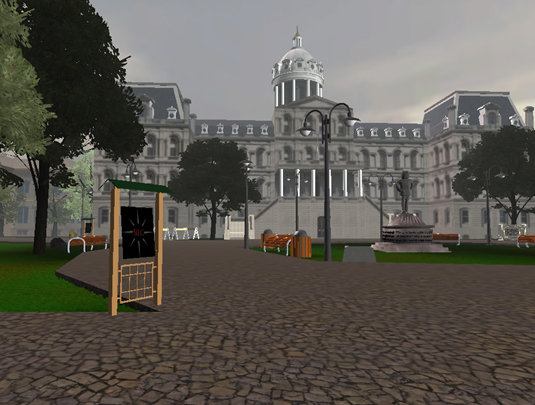
\includegraphics[width=12cm,height=6cm]{./figs/Cover_Page.jpg}\\[\bigskipamount]

\begin{figure}[!htb]
\minipage{0.32\textwidth}
  
\includegraphics[width=\linewidth]{./figs/Temple.jpg}
  \caption*{}\label{fig:awesome_image1}
\endminipage\hfill
\minipage{0.32\textwidth}
  
\includegraphics[width=\linewidth]{./figs/SILC.jpg}
  \caption*{}\label{fig:awesome_image2}
\endminipage\hfill
\minipage{0.32\textwidth}%
  \includegraphics[width=\linewidth]{./figs/SCANN_LAB.png}
  \caption*{}\label{fig:awesome_image3}
\endminipage
\end{figure}

\end{center}
}
\ifluatex
  \usepackage{selnolig}  % disable illegal ligatures
\fi
\usepackage[]{natbib}
\bibliographystyle{apalike}

\title{Virtual Silcton Documentation}
\author{Steven M. Weisberg, PhD}
\date{21 August, 2020}

\begin{document}
\maketitle

{
\hypersetup{linkcolor=}
\setcounter{tocdepth}{1}
\tableofcontents
}
\setstretch{1.5}
\hypertarget{virtual-silcton-introduction}{%
\chapter{Virtual Silcton Introduction}\label{virtual-silcton-introduction}}

Welcome to the documentation for \textbf{Virtual Silcton}.

The Virtual Silcton environment was originally designed in \href{https://unity.com/}{Unity3D} by \href{vschinaz@bond.edu.au}{Victor Schinazi} and Drew Dara-Abrams. In 2011, Steven Weisberg began updating and maintaining the documentation and website for administration of the Virtual Silcton environment.

This documentation was drafted by \href{scannlab.psych.ufl.edu}{Steven M. Weisberg} and last edited on the date at the top of this page.

\begin{figure}
\centering
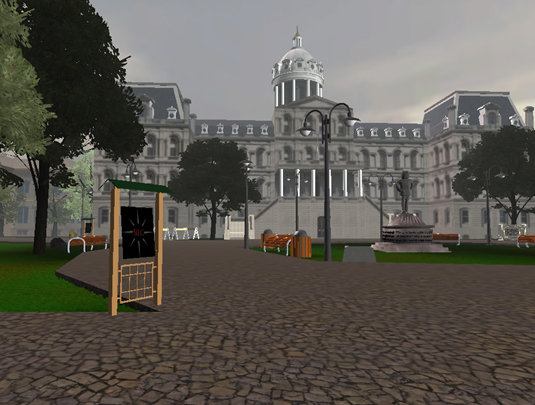
\includegraphics{./figs/Cover_Page.jpg}
\caption{Virtual Silcton Image}
\end{figure}

\hypertarget{virtual-silcton-background}{%
\chapter{Virtual Silcton Background}\label{virtual-silcton-background}}

\hypertarget{experimenter-interface}{%
\chapter{Experimenter Interface}\label{experimenter-interface}}

\hypertarget{labs}{%
\section{Labs}\label{labs}}

\hypertarget{experimenters}{%
\section{Experimenters}\label{experimenters}}

\hypertarget{studies}{%
\section{Studies}\label{studies}}

\hypertarget{active-vs.-inactive}{%
\section{Active vs.~Inactive}\label{active-vs.-inactive}}

\hypertarget{participant-ids}{%
\section{Participant IDs}\label{participant-ids}}

\hypertarget{building-studies}{%
\chapter{Building Studies}\label{building-studies}}

\hypertarget{administering-to-participants}{%
\chapter{Administering to Participants}\label{administering-to-participants}}

\hypertarget{participant-instructions}{%
\chapter{Participant Instructions}\label{participant-instructions}}

\hypertarget{data-analysis-tips-and-scripts}{%
\chapter{Data Analysis Tips and Scripts}\label{data-analysis-tips-and-scripts}}

\hypertarget{onsite-pointing-data}{%
\section{Onsite Pointing data}\label{onsite-pointing-data}}

\hypertarget{navigation-logs}{%
\section{Navigation Logs}\label{navigation-logs}}

\hypertarget{model-building-tasks}{%
\section{Model Building Tasks}\label{model-building-tasks}}

  \bibliography{book.bib,packages.bib}

\end{document}
